\section{The shape of the tight state, and two predictions}\label{sec:shape}

\subsection{The notched heptagon}
The outline of the folklore state is as simple as an outline can be. At the regular pentagon $P^*$ the boundary of the core has exactly five sides (three creases and two band edges), and every side direction lies in the lattice $36^\circ\mathbb{Z}$; the picture one draws by hand is the picture the model produces (Figure~\ref{fig:pentagon} in Section~\ref{sec:moduli}). At $\td$ the side directions leave that lattice and the outline acquires two further sides. They are small, and they are the whole point: together they cut a notch into one edge.

\begin{proposition}[Shape of $\td$]\label{prop:heptagon}
The core silhouette of $\td$---the boundary of the four passes with $A$ cut at $\ell_2$ and $D$ cut at $y=0$, in the same flush-cut convention as the truncation length---is a mirror-symmetric heptagon $E\,H\,G\,K\,X\,Y\,F$ with exactly one reflex vertex. Here $K=Q_1=I$ is the endpoint of the crease $\kappa_3$ that sits on the far edge $e_B$ of the lay-in band (the active wall $w_5$), while $X=Q_0$ is the other endpoint of $\kappa_3$, and $Y$ is the intersection of $e_B$ with the far edge of the lay-out band. The seven sides measure
\[
|EH|=|GK|=h^\dagger=a^\dagger=1.036386,\qquad |FE|=|KX|=1.050603,
\]
\[
|HG|=1.061053,\qquad |XY|=|YF|=0.051419,
\]
the last two forming a mirror pair of micro-sides carried by the lay-out and the lay-in edge. The interior angles are
\[
\angle E=\angle K=\angle X=\angle F=107.855^\circ,\qquad \angle H=\angle G=109.531^\circ,
\]
together with the reflex angle $\angle Y=249.517^\circ$; they sum to $900^\circ$, as a heptagon requires. The open triangle $XYF$ is covered by none of the four passes: the outline carries a genuine V-notch, cut into one edge and centred on the mirror axis (Figure~\textup{\ref{fig:heptagon}}).
\end{proposition}

\begin{proof}
The seven vertices are rational functions of the coordinates of $\td$. Their squared distances, and the angle cosines after the stated simplifications, admit exact algebraic certificates; the displayed lengths and angles in degrees are rounded evaluations, not claims that angle measures belong to $\Q(x^\dagger)$.

Here is a certificate for the \emph{whole} silhouette. The four flush-cut panels are
\begin{gather*}
A=[E,F,K,G],\quad B=[E,H,G,F],\\
C=[H,G,K,X],\quad D=[X,K,H,E].
\end{gather*}
Exact convex clipping, vertex containment and area identities give
\[
A\cup B=[E,H,G,K,F],\qquad C\cup D=[E,H,G,K,X],
\]
whose intersection is the convex pentagon $I=[E,H,G,K,Y]$.
Their union is $I\cup[E,Y,F]\cup[K,X,Y]$; the three pieces have disjoint interiors. Cancelling their shared edges leaves the simple boundary $EHGKXYF$. Exact orientation tests exclude intersections of nonadjacent boundary edges and show that only $Y$ is reflex. All signs use rational interval evaluation around a Sturm-isolated root of $p_x$; equalities are reduced modulo $p_x$. These are full polygon certificates, not tests at edge midpoints (\texttt{exact\_outline}).

The open triangle $XYF$ also misses the \emph{untruncated} passes. For each pass there is a containing closed half-plane, bounded respectively by $KF$, $GF$, $XH$ and $XE$, whose inward linear functional has signs at $(X,Y,F)$
\[
A:(-,0,0),\quad B:(-,-,0),\quad
C:(0,-,-),\quad D:(0,0,-).
\]
Every point of the open triangle is a strictly positive barycentric combination of its vertices. Each functional is therefore strictly negative there, proving noncoverage by every infinite pass, including both tails.
\end{proof}

\begin{proposition}[The exact notch data]\label{prop:notch}
The squared mouth $|XF|^2$, the squared legs $|XY|^2=|YF|^2$, the squared depth, and the cosine of the reflex angle are elements of $\Q(x^\dagger)$, given by the following polynomials evaluated at $x=x^\dagger$:
\begin{align}
\mathrm{mouth}^2&=-\tfrac{x^{10}}{6}-\tfrac{11x^8}{12}-\tfrac{5x^6}{4}-\tfrac{7x^4}{12}+\tfrac{7x^2}{4}-\tfrac16,\label{eq:notch-mouth}\\
\mathrm{leg}^2&=-\tfrac{x^{10}}{48}-\tfrac{x^8}{6}-\tfrac{5x^6}{24}-\tfrac{x^4}{3}+\tfrac{x^2}{16},\label{eq:notch-leg}\\
\mathrm{depth}^2&=\tfrac{x^{10}}{48}+\tfrac{x^8}{16}+\tfrac{5x^6}{48}-\tfrac{3x^4}{16}-\tfrac{3x^2}{8}+\tfrac1{24},\label{eq:notch-depth}\\
\cos\angle Y&=-\tfrac{x^{10}}{24}-\tfrac{x^8}{8}+\tfrac{x^6}{8}-\tfrac{11x^4}{24}-\tfrac{11x^2}{12}-\tfrac14.\label{eq:notch-angle}
\end{align}
All four polynomials are even, so, exactly as for the multiplier $\lambda_{w_5}$ of Theorem~\textup{\ref{thm:kkt}}, the four displayed quantities lie in the sextic subfield $\Q((x^\dagger)^2)$ rather than in the full degree-twelve field. Numerically, for a strip of width $w$,
\begin{gather*}
\mathrm{mouth}=0.0844877\,w,\qquad \mathrm{leg}=0.0514189\,w,\\
\mathrm{depth}=0.0293149\,w,\qquad \angle Y=249.5170066^\circ.
\end{gather*}
\end{proposition}

\begin{proof}
The seven vertices are rational functions of $\td$, so each squared length is a rational expression in $x^\dagger$; reducing it in the quotient field $\Q[x]/(p_x)$ returns the canonical representatives \eqref{eq:notch-mouth}--\eqref{eq:notch-angle}. Two identities in that quotient are worth recording, since they are what makes the notch a notch. The mirror identity $|XY|^2-|YF|^2$ reduces to exactly $0$, which is also why $\cos\angle Y$ is a field element rather than an expression involving a square root; and the isosceles Pythagorean relation $\mathrm{depth}^2=\mathrm{leg}^2-(\mathrm{mouth}/2)^2$ holds identically, an internal check on four representatives computed independently of one another.
\end{proof}

\begin{figure}[t]
\centering
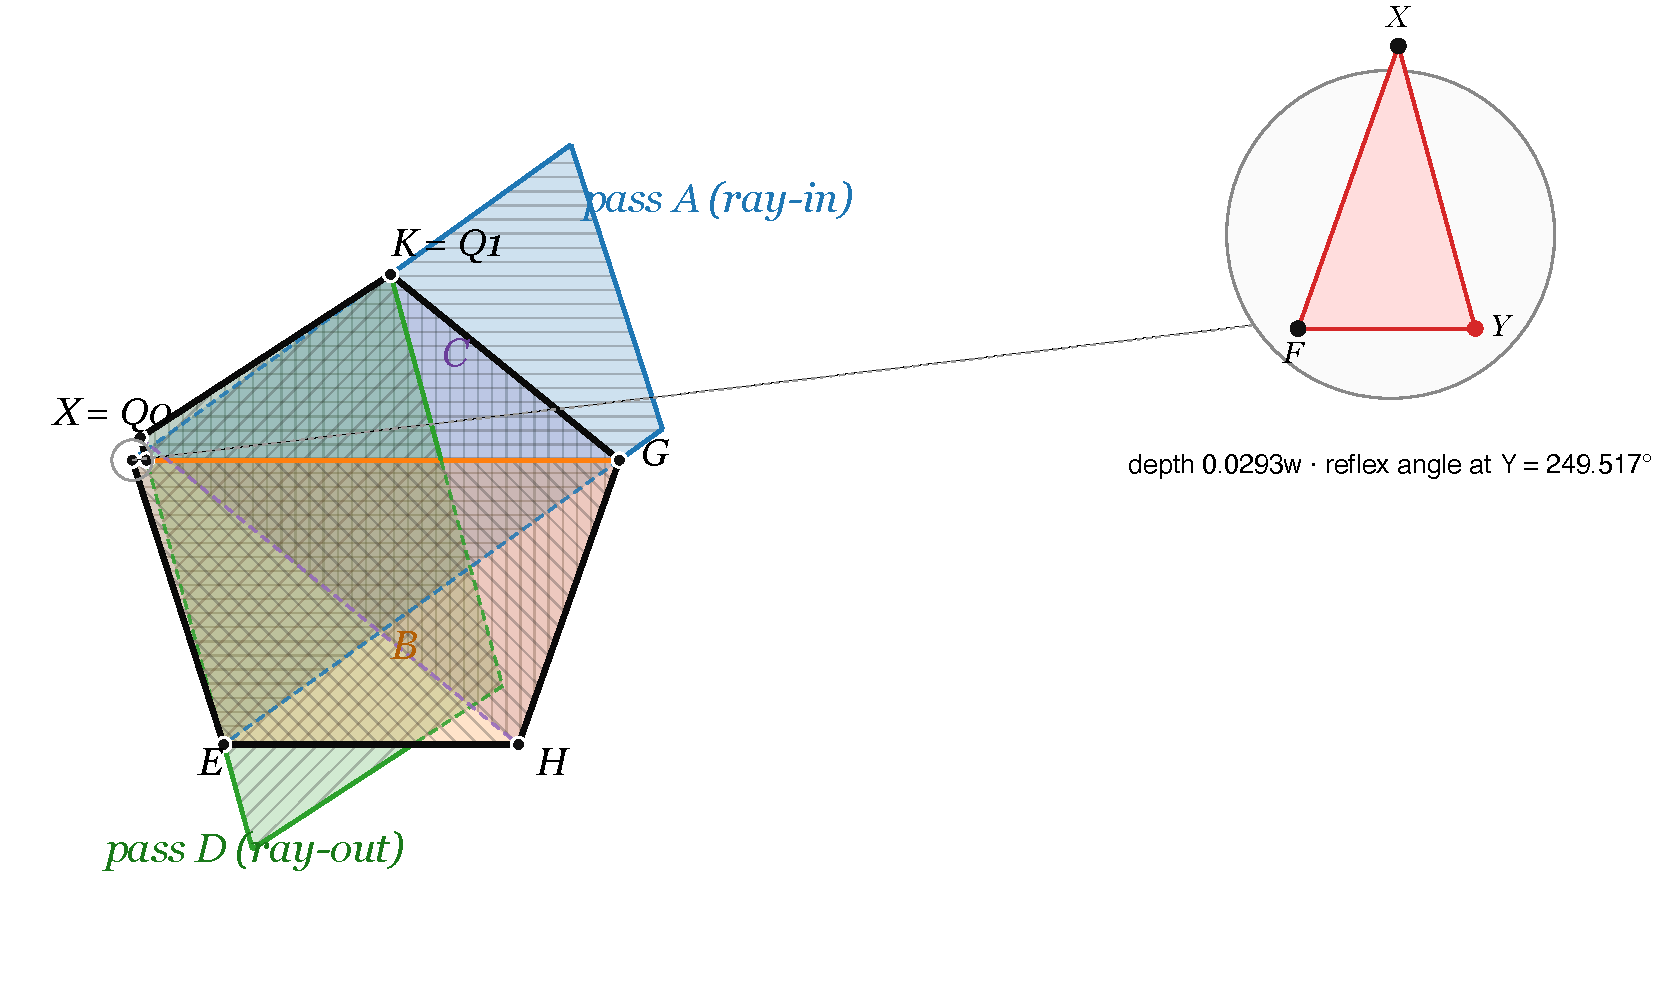
\includegraphics[width=0.95\linewidth]{figs/fig2-heptagon.pdf}
\caption{The tight state $\td$, rendered in the hidden-line convention (solid edges visible, dashed edges passing beneath; creases are the heavy red chords): the mirror-symmetric notched heptagon $E\,H\,G\,K\,X\,Y\,F$, with the V-notch straddling the mirror axis, enlarged in the inset---mouth $0.0845\,w$, legs $0.0514\,w$ for strip width $w$---and quantified exactly in Proposition~\ref{prop:notch}. Compare the five-sided outline of Figure~\ref{fig:pentagon}.}
\label{fig:heptagon}
\end{figure}

\begin{remark}[Contact saturation and symmetry]\label{rem:flushness}
At $P^*$ the eight-wall junction has dihedral symmetry. At the core-length minimum $\td$, Proposition~\ref{prop:heptagon} gives a notched heptagon and Theorem~\ref{thm:s6} gives the associated sextic group $S_6$. Thus tightness alone does not force a regular polygon.
\end{remark}

\begin{remark}[The notch mouth \emph{is} the crease clearance]\label{rem:mouth-clearance}
The mouth $|XF|$ of the notch and the crease clearance $c_{\mathrm{cr}}(\td)=d(\kappa_1,\kappa_3)$ are the same segment. Indeed $X=Q_0$, and the taco parameters at $\td$ satisfy $t=u=1.0506>1$: the intersection of the two crease \emph{lines} lies beyond both crease \emph{segments}, so the minimum distance between $\kappa_1$ and $\kappa_3$ is attained at the endpoint pair $(F,Q_0)$, with both feet at parameter $1$ and the two quantities agreeing to machine precision. This closes a circle with the six-wall identity of the standard slice (Observation~\ref{obs:corner}): on the slice the two creases touch at the shared corner $Q_0=F$, the crease clearance vanishes and the taco pair vanishes identically; moving along the second family opens that contact; and the notch mouth measures precisely how far it has opened by the time tightening stops. In this sense the notch is not a blemish on the tight shape but the geometric record of the descent that produced it.
\end{remark}

\subsection{Two predictions}
In core length the pentagonal and dagger states differ by only $0.114\%$, requiring careful control of material and measurement effects to resolve experimentally. The V-notch provides a second observable. The following predictions refer to the kinematic model.

\begin{remark}[Prediction (i): the notch]\label{rem:pred-notch}
\emph{Within the kinematic model}, the certified pulling path terminates not at the pentagon but at the notched heptagon $\td$ of Theorem~\ref{thm:sosc}, with the four exact quantities of Proposition~\ref{prop:notch}: mouth $0.0845w$, legs $0.0514w$, depth $0.0293w$, and reflex angle $249.52^\circ$. On a $2\,\mathrm{cm}$ tape this is a notch about $1.7\,\mathrm{mm}$ wide and $0.6\,\mathrm{mm}$ deep, visible to the eye and straightforward to measure. Real paper may instead lock at the pentagon: friction at eight simultaneous contacts, creases pinned by the material rather than free to move, or a thickness cost exceeding the $0.114\%$ core gain would each arrest the descent at the pass. Measuring the notch distinguishes the predicted outlines of the two optima.
\end{remark}

\begin{remark}[Prediction (ii): a slab-construction cost]\label{rem:pred-thickness}
Along one certified opening direction, our constant-height hairpin construction realizes nearby open states at cost
\[
\Delta\ell\;\approx\;\Bigl(\sum_j\lambda_{w_j}\Bigr)t(\varepsilon)\;\lesssim\;3.5\,\varepsilon .
\]
The reasoning is a first-order trade between two linear rates along the opening direction $\delta$ of Lemma~\ref{lem:opening}. On one side, the KKT identity of Theorem~\ref{thm:kkt} turns the cost of opening into the sum of the multipliers,
\[
\core(\theta_t)-\ell^\dagger=(\nabla\core\cdot\delta)\,t+O(t^2)=\Bigl(\sum_j\lambda_{w_j}\Bigr)t+O(t^2)\approx4.11\,t;
\]
on the other, the realizable slab budget grows linearly from zero along the same path, $\varepsilon_0(\theta_t)\approx1.16\,t$, so a state realized by \emph{this construction} in a slab of height $\varepsilon$ sits at $t\gtrsim\varepsilon/1.16$ along the path. Combining the two rates gives the stated law. Its interpretation is the content of the prediction: \emph{the KKT multipliers are the unit prices of the ramp clearances}. Each active wall is a clearance that tightening has spent, and $\lambda_j$ is the core length bought per unit of clearance handed back, which is why the coefficient is a sum of multipliers and not a geometric constant. Two caveats. This is an $O(\varepsilon)$ \emph{upper} bound produced by one particular opening path; the matching lower bound is not established, and a different slab realization might do better than anything on that path. And the coefficient $3.5$ inherits the numerical status of $\varepsilon_0$, whereas $\sum_j\lambda_{w_j}$ is exact.
\end{remark}

\begin{remark}[Static realization is not dynamic tightening]\label{rem:static-dynamic}
Theorem~\ref{mainthm:realization} lifts \emph{individual} states into slabs, one $\varepsilon$ at a time. Lifting an entire tightening path into a \emph{single} slab of fixed height is a different statement, and it is not proved here; it is posed as open problem~\ref{op:lifting} below. Both predictions should be read with that gap in view.
\end{remark}

\section{Toward global uniqueness: a stratified census}\label{sec:census}

Everything established so far is local. Theorem~\ref{thm:sosc} makes $\td$ a strict local minimizer of $\core$ and Theorem~\ref{thm:pass} makes the pentagon a pass, but neither excludes a further blocked state elsewhere in $\M$. This section closes that gap as far as we can, in two stages: first a descent census, which is evidence, and then a stratified census of first-order blocked points, which is a classification carrying per-candidate certificates.

\begin{remark}[Descent census]\label{rem:descent-census}
Three independent multistart sweeps (different seeds, perturbations of size $\pm0.03$ to $\pm0.20$ around slice states with $x\in[0.10,0.32]$) produced $286$ valid starting points, and all $286$ converged to the single attractor $\td$, with terminal spread at most $1.2\times10^{-7}$ and $|\ell-\ell^\dagger|\le2.3\times10^{-13}$. Every terminal active set was exactly $\{w_1,w_4,w_5,w_6\}$. No local minimum other than $\td$ was found, and no run stalled at the pentagon corner: random descent passes straight through the pass, a dynamical reproduction of Theorem~\ref{thm:pass}.
\end{remark}

The coverage of Remark~\ref{rem:descent-census} has three limits. The region $x<0.10$ was not sampled; strata on which a taco wall is active cannot be reached by this method, since they lie far from the sampled region; and starts placed on the boundary strata themselves were not tested. An independent verification pass reproduced a sample of the descents and extended the coverage with distant probes (valid starting points at max-norm distance $4.7$ from the slice), which again reached $\td$. This is strong numerical evidence for global uniqueness; it is not a proof, and the route to one is symbolic elimination over the remaining strata (open problem~\ref{op:uniqueness}).

The classification replaces descent by first-order blocking. Recall that a valid state is \emph{blocked} when $\nabla\core$ lies in the cone generated by the gradients of the walls active at it, taken within the relevant branch of the disjunctive taco pair: the first-order statement that no feasible direction decreases the core length. Blockedness is what tightening produces, and it is independent of how, or whether, a state is reached. Its relation to the active-set geometry is governed by the constraint qualification in force, and here the taco pair rules out the stronger of the two standard ones.

Recall Observation~\ref{obs:corner}: $w_9=w_{10}=0$ exactly when $Q_0=F$, a three-dimensional locus $\mathcal F$ on which the four active wall gradients have rank two, so LICQ fails identically. The locus meets the valid region, and the standard symmetric slice is exactly $\mathcal F\cap\{w_1=w_4=0\}$. Numerically, the valid locus on which six or more walls are active consists of the slice and the pentagon alone.

Because LICQ fails on $\mathcal F$, the census is formulated under the weaker Mangasarian--Fromovitz condition (MFCQ): the existence of a direction strictly increasing every wall active on the relevant taco branch \cite{nocedal2006}.

\begin{theorem}[Stratified census; $=$ Theorem~\textup{\ref{mainthm:census}}]\label{thm:census}
Let $\theta$ be a tight state at which MFCQ holds for the relevant taco branch. Then $\theta$ is blocked; and by the cone form of Carath\'eodory's theorem every blocked point solves the square KKT system of an active set $S$ with $|S|\le5$ containing at most one taco wall. The enumeration runs over all active sets of size at most five, both-taco sets included as redundant super-captures, less the four subsets of $\{w_4,w_6\}$ excluded by the $x$-independence lemma: $215$ strata, capturing all candidates, including those sitting at high-activity corners. Across all $215$ strata the only \emph{certified} surviving blocked state is $\td$; the residual components are computational and are itemized in the proof and in Table~\ref{tab:census}. The pentagon occurs as a root of the KKT system in twenty of them and is excluded in each by the single exact Farkas certificate of Theorem~\textup{\ref{thm:pass}} together with cone monotonicity.
\end{theorem}

\begin{proof}[Proof of Theorem~\textup{\ref{thm:census}}]
\emph{Tight and MFCQ imply blocked.} Suppose a tight state $\theta$ is not blocked on its taco branch. By the Farkas alternative there is a direction $d$ with $\nabla\core\cdot d<0$ and $\nabla w_i\cdot d\ge0$ for every active wall $i$; MFCQ supplies $e$ with $\nabla w_i\cdot e>0$ for all active $i$, and $\tilde d=d+\eta e$ with $\eta>0$ small satisfies $\nabla\core\cdot\tilde d<0$ and $\nabla w_i\cdot\tilde d>0$ simultaneously. For small $t>0$ the segment $\theta+t\tilde d$ then keeps every active wall strictly positive by first-order Taylor expansion, keeps the inactive walls and the (open) branch conditions by continuity, and strictly decreases $\core$: a pulling path issuing from $\theta$ that decreases the core length, contradicting tightness. On the taco union the argument is applied on each branch separately.
The grades inside the statement are not uniform, and the split is worth spelling out. The \emph{reduction} is proved. MFCQ is certified exactly at $P^*$ and at $\td$: rank-$4$ LICQ at $\td$, by a $4\times4$ minor of the active-gradient matrix that is nonzero in $\Q[x]/(p_x)$, and at the pentagon an explicit rational direction whose eight wall derivatives are rigorously positive under interval evaluation. The Carath\'eodory step is a theorem about cones \cite{barvinok2002}, and it is what licenses the truncation to $|S|\le5$ and to at most one taco wall: strata with both taco walls active are redundant super-captures of strata already on the list, so no candidate escapes through them. The \emph{arithmetic} is exact as well. All eight wall functions admit $\mathbb{Z}$-coefficient polynomial representatives, of degrees $(2,16,4,16,4,16,5,3)$ in the order $(w_1,w_4,w_5,w_6,w_7,w_8,w_9,w_{10})$, and $\core=(x+g+h+a+b)/2$ is affine. Clearing the wall denominators on their nonzero sign domains therefore gives a polynomial KKT system for each stratum. Polynomialization multiplies each wall by a scale factor whose sign is itself part of the bookkeeping: it is positive unconditionally for $w_1,w_4,w_6,w_7,w_8$, and only on the relevant branch for $w_5,w_9,w_{10}$. In the variable $q=g-h$, the final encoding uses $c_5=(q+x)(1-qx)$ but $c_7=(q^2+1)(x^2+1)>0$; the latter requires no extra sign condition. The certificates accordingly either use the unconditional walls alone or co-certify the scale. The census is run over the computational chamber $\Mhat$; its stratum systems are domain-free polynomial systems and no recorded disposition invokes the taco sign, so the dispositions read verbatim over the honest moduli; within the computational harvest, the extra honest region $\{t\le0\}\cup\{u\le0\}$ produced no harvested candidate---per-stratum completeness of the harvest remaining, as elsewhere, a numerical component.

Two exact exclusions simplify the census. The second excludes particular roots, not whole strata. Those with $S\subseteq\{w_4,w_6\}$ carry no blocked point at all, because $w_4$ and $w_6$ are independent of $x$ while $\partial\core/\partial x\equiv\frac12$ globally; and every occurrence of the pentagon as a KKT root is excluded by the Farkas certificate of Theorem~\ref{thm:pass}. On the stratum $\{w_1,w_4,w_5,w_6\}$ the unique KKT point is $\td$ itself, by the reduction to the plane curve $N_5$ and the minimal polynomial $p_x$. That leaves $104$ harvested candidates elsewhere. Of these, all $72$ that admit a certifiable regular root carry per-candidate Krawczyk root enclosures together with interval-sign exclusions on those root-isolating boxes---using unconditionally scaled walls, scale-co-certified conditional walls, or direct interval evaluation of a true wall (in fact, \texttt{exact\_census\_roots} freshly isolates all $72$ roots in $100$-digit \textsc{Arb} ball arithmetic and certifies that every one violates a true geometric sliver wall strictly below $-0.315$ on its isolated root box)---and those exclusions are rigorous.

\begin{compres}[The numerical residue, localized]\label{compres:residue}
For the remaining $32$ candidates the Krawczyk operator is inconclusive, so whether a genuine stratum root exists near them remains open. Classifying their saved approximate centres gives four with $x<0$, six with $|q+x|<10^{-6}$, eighteen with $|1-qx|<10^{-6}$ (the second factor of the $w_5$-denominator $c_5=(q+x)(1-qx)$), and four remaining centres (all with $h,a<0$); none satisfies $q+x=0$ or $1-qx=0$ exactly as stored decimals. At radius $10^{-12}$ around every one of the $104$ saved centres, a true sliver wall is certified below $-0.315$ in both \textsc{Arb} and \texttt{mpmath} interval arithmetic (the reported maximum active-wall residual of $19.5$ occurring at a floating-point denominator of order $2.1\times10^{-15}$). Beyond this, the numerical residue of Theorem~\ref{thm:census} is confined to three isolated components: the per-stratum completeness of the harvest, that is, that no real root of a stratum's KKT system was missed by multistart; the absence of valid states at which MFCQ fails, verified numerically on $\mathcal F$; and the calibration of the on-branch multiplier scales. Each has a concrete symbolic route, described in open problem~\ref{op:uniqueness}. The completeness component is doubly implemented: two independent constructions of the wall system, rational expression trees with $30$ seeds per stratum and polynomialized walls with $100$, return identical outcomes, with $\td$ the only candidate passing every filter in both. For reference, the chart-coordinate wall representatives are compact: with $q=g-h$, the wall $w_1$ has integer representative $2gx+x^2-1$ over denominator $1$; the walls $w_4,w_6,w_8$ share the manifestly positive denominator $(q+a-b)^2+1$ and $w_7$ the denominator $q^2+1$, with quartic numerators; $w_5$ has the branch-signed denominator $(q+x)(qx-1)$, the census scale factor $c_5$ up to sign; and the taco pair shares one cubic denominator, the line-pair determinant of $\kappa_1,\kappa_3$, with $w_{10}$'s numerator equal to $b\,(q^2+2qx-1)+h\,(q^2+1)$. The degrees quoted above are those of the \emph{eliminated} polynomializations used by the census, not of these chart representatives; both encodings, in machine-readable form, are \texttt{uniq\_setup} and \texttt{uniq\_poly} in the suite. The sixty-seven archived sliver-sign exclusions (and seventy-one wall exclusions in a fresh run) are additionally re-verified in the ball arithmetic of \textsc{Arb} (\texttt{arb\_recheck}), independently of \texttt{mpmath}. Table~\ref{tab:census} collects the split.
\end{compres}
\end{proof}

\begin{table}[t]
\centering\small
\begin{tabular}{@{}p{0.56\linewidth}l@{}}
\hline
Ingredient of Theorem~\ref{thm:census} & Status\\
\hline
\raggedright Tight and MFCQ imply blocked; MFCQ certificates at $P^*$ and $\td$ & exact\tabularnewline
\raggedright Carath\'eodory reduction to $|S|\le5$ with at most one taco wall & proof\tabularnewline
\raggedright Wall polynomialization, rationality of $\core$, the manifold $\mathcal F$ & exact\tabularnewline
\raggedright Emptiness of the strata $S\subseteq\{w_4,w_6\}$; exclusion of all pentagon root copies & exact\tabularnewline
\raggedright Uniqueness of $\td$ on the stratum $\{w_1,w_4,w_5,w_6\}$ & exact\tabularnewline
\raggedright Exclusion of the $72$ candidates with certifiable regular roots & interval\tabularnewline
\raggedright Exclusion of the $32$ candidates with inconclusive Krawczyk operator & numerical\tabularnewline
\raggedright Per-stratum completeness of the harvest; absence of valid non-MFCQ points; on-branch scale calibration & numerical\tabularnewline
\hline
\end{tabular}
\caption{Verification grades inside the stratified census. Here \emph{exact} means symbolic computation in $\Q$, $\Q(\sqrt5)$, or $\Q[x]/(p_x)$; \emph{interval} means a machine-checked enclosure argument; and \emph{numerical} means floating-point evidence with the residue localized as stated.}
\label{tab:census}
\end{table}

Two closing remarks on what the census does and does not say. It classifies \emph{blocked} points, so it is insensitive to reachability: descent along the certified path of Theorem~\ref{mainthm:pass} reaches $\td$, while the behaviour of generic descent remains the numerical statement of Remark~\ref{rem:descent-census}. And it is a classification of first-order behaviour only; the strictness of the minimum at $\td$ comes from the exact reduced Hessian of Theorem~\ref{thm:sosc}, not from anything in this section.

\section{Beyond the trefoil: an exact blocked hexagon for the figure-eight knot}\label{sec:figure8}

Everything so far concerns the unique three-crease branch. This section runs the same program---enumerate, build the moduli space, tighten, identify, certify---one crossing higher, and proves Theorem~\ref{mainthm:hex}. The outcome is a second data point for the general theory, and a striking one: where the trefoil produced a degree-twelve certified minimizer outside the reach of radicals, the figure-eight produces a certified blocked minimizer in a quadratic field.

\subsection{The branch}
Running the enumeration machinery of Theorem~\ref{mainthm:fold} at four creases (block-ordered cyclic codes, Gauss parity, planarity of the rotation systems) yields exactly one irreducible four-crossing code, $\mathtt{XYZXWZYW}$ in the crossing alphabet of Section~\ref{sec:model}, with exactly two planar rotation systems forming a mirror pair. Evaluating the Kauffman bracket over all sixteen over/under assignments shows that exactly two produce the Jones polynomial of the figure-eight knot $4_1$ (a mirror pair, as amphichirality requires), two that of the trefoil, and twelve that of the unknot. The naming does not rest on the Jones polynomial, which is not a complete invariant. The shadow code of the branch and the shadow code of the standard figure-eight diagram canonicalize to the same cyclic word; the shadow admits exactly two planar rotation systems, a mirror pair; and the two surviving assignments are precisely the two alternating decorations of that shadow. Hence the two decorated diagrams \emph{are} the standard figure-eight diagram and its mirror, up to homeomorphism of the plane, and the knot is $4_1$ by definition; the bracket computation is the search that isolated them. The figure-eight is therefore the unique new knot arising from the irreducible four-crossing code---codes with five or six crossings, permitted at $n=4$ by the crossing bound, are enumerated combinatorially but their knots are not classified here---and it determines a branch $\mathcal B_{4_1}$ whose centreline chart $(\tau_1,\ldots,\tau_4,L_1,L_2,L_3)$ has dimension $2n-1=7$, in agreement with the dimension count of Proposition~\ref{prop:dim}.

A long diagram cuts the closed code at a base point and distributes the eight crossing visits among five straight passes $P_0,\ldots,P_4$; a \emph{cell} of the branch records which pass pairs cross and under which layer order (Figure~\ref{fig:f8code}). Two constraints prune the combinatorics before any geometry is computed: a straight pass can cross only non-adjacent passes, and the over/under pattern of a $4_1$ assignment must extend to a total layer order, that is, the pairwise above/below relations it forces must be acyclic. A rerun of $8\times10^6$ sampled configurations with the actual crease-capped panel oracle found the candidate cell: \emph{the figure-eight knot does fold flat at width one with four creases}, and every valid state found---$21$ distinct states, each recorded twice, once for each top--bottom flip---lies in a single cell, with crossing pairs $\{(0,2),(0,3),(1,4),(2,4)\}$, self-mirror under material reversal, and layer order $P_1>P_4>P_2>P_0>P_3$ up to the flip; the two flip records per state are an accounting identity, not an observation. The rerun uses eight independent random streams with seeds $7000,\ldots,7007$, each generating $10^6$ configurations with the turn magnitudes sampled uniformly from $[0.3,3.1]$ and the three lengths from $[0.3,4.0]$. Half the sign-pattern draws choose a common turn sign, and half choose four independent signs. The oracle tests the actual oblique crease caps, unbounded tails, the layer axiom, and centreline general position; its source snapshots, tolerances, seeds and all accepted states are recorded by \texttt{n4\_rerun}. The turn sign pattern is $(+,+,-,-)$: where the tightened trefoil winds as a spiral, the figure-eight folds as a point-symmetric zigzag, the geometric expression of its amphichirality. Existence has since been upgraded to exact---the state $\theta^*_{4_1}$ of Theorem~\ref{mainthm:hex} is itself certified valid, all six forbidden crease/pass intersections tested against the actual convex panels by exact affine half-plane clipping in $\Q(\sqrt{15})$ (\texttt{n4\_exact\_valid})---while the exhaustiveness of the cell remains a numerical statement, graded as such (Figure~\ref{fig:f8loose}).

\begin{figure}[t]
\centering
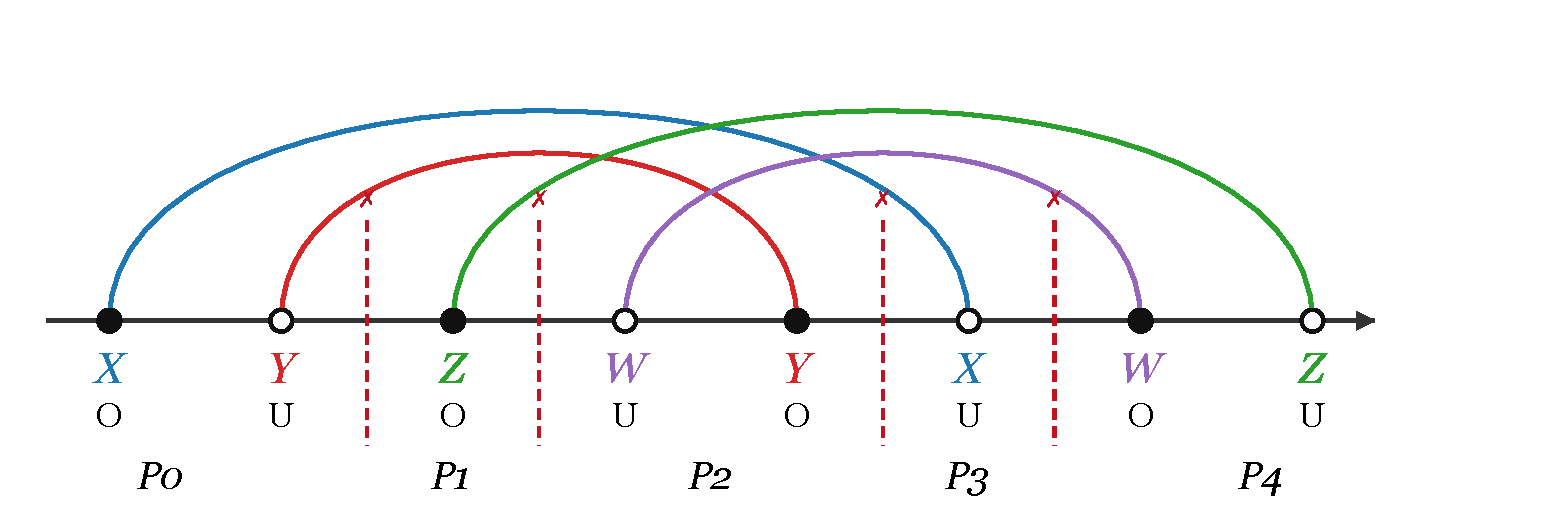
\includegraphics[width=0.9\linewidth]{figs/fig41-code.pdf}
\caption{The realized cell as combinatorics. The material line carries one rotation of the canonical code, with the crossings relabelled, read $X\,Y\,Z\,W\,Y\,X\,W\,Z$, with the alternating over/under pattern of the $4_1$ assignment (filled = over); the four cuts (dashed) distribute the eight visits into the passes $P_0,\dots,P_4$, producing the crossing pairs $X\colon(0,3)$, $Y\colon(0,2)$, $Z\colon(1,4)$, $W\colon(2,4)$ of the cell, with layer order $P_1>P_4>P_2>P_0>P_3$.}
\label{fig:f8code}
\end{figure}

\begin{figure}[t]
\centering
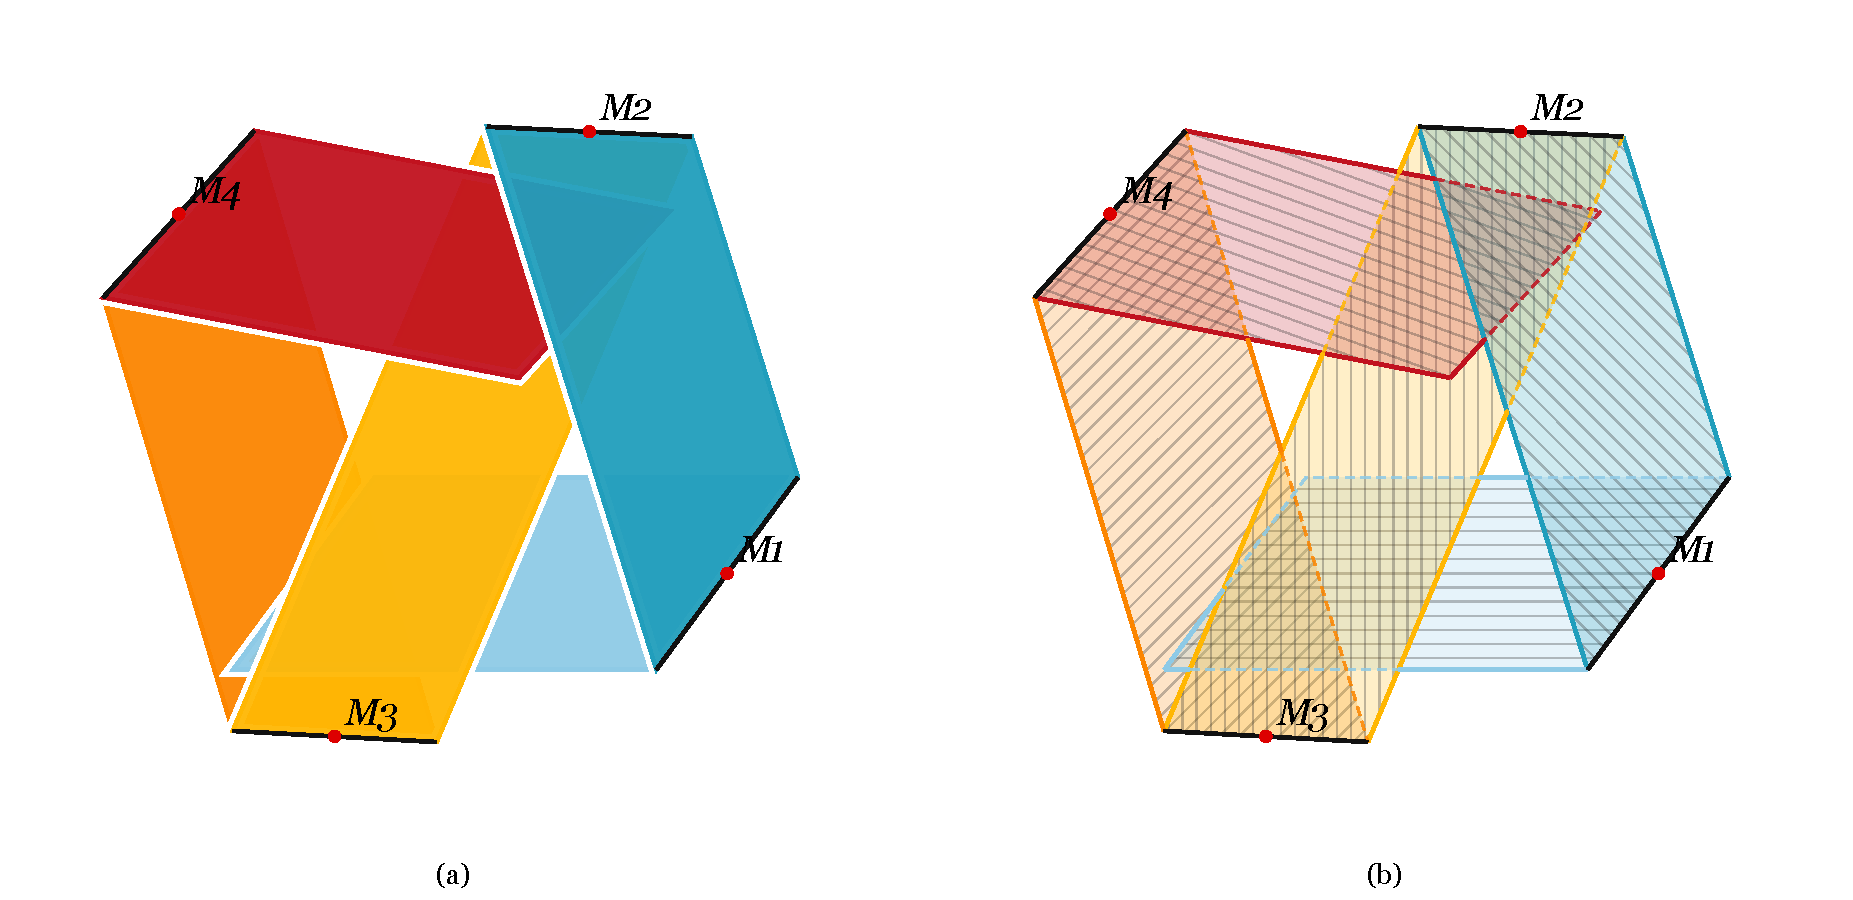
\includegraphics[width=\linewidth]{figs/fig41-loose.pdf}
\caption{A valid width-one flat folded figure-eight state before tightening ($\core\approx8.65$): (a) the state as seen from above; (b) its structure, dashed edges passing beneath. Fold points $M_1,\ldots,M_4$ are marked; crease chords are the heavy segments; the two rays are the tails. The weave is the point-symmetric zigzag cell described in the text.}
\label{fig:f8loose}
\end{figure}

The crossing shadow alone can admit an unknot layering at $\core\approx2.66$. Among its sixteen assignments the integer determinants are $1$ (twelve times), $3$ (twice) and $5$ (twice). A Fox five-colouring count of $25$ selects precisely the figure-eight pair. For the crease-neighbourhood condition, the half-planes of each actual pass pull back to affine inequalities along a crease. Intersecting the resulting parameter intervals tests its full relative interior. A grid of $31$ points can miss a penetration of depth $0.031$ in the final three percent of a chord, admitting an apparent minimum $0.096$ below the certified contact-chamber candidate. The search uses the interval-intersection rule with explicit floating-point tolerances. The point and opening certificates use ordered algebraic fields.

\subsection{The tight state, exactly}
Fixing the layer order, the corrected-oracle rerun descends $\core=L_1+L_2+L_3$ from all $42$ state--layering records. With the recorded finite search budget, $31$ endpoints have core length within $0.01$ of $4\sqrt{15}/3$; this threshold measures proximity in objective value, not certified convergence in configuration space. At each of the other $11$ endpoints, a linear-programming direction followed by $101$ actual-panel checks along a short ray gives a numerically feasible decrease. These sampled rays are evidence of optimization stalls, not interval-certified continuous paths or a complete Farkas classification. The exact state identified from this search is symmetric under material reversal, $\tau_4=-\tau_1$, $\tau_3=-\tau_2$, $L_3=L_1$, and its active set consists of eight contacts of exactly the kind the trefoil walls led us to expect: the endpoints of crease chords $1$ and $4$ against the bands of the passes between them in the layer order, and---the new feature---crease chords $2$ and $3$ lying \emph{parallel along} a band edge, a corner contact in which both chord endpoints touch simultaneously. On the symmetric slice these eight conditions reduce to four equations in $(\tau_1,\tau_2,L_1,L_2)$, a zero-dimensional square system. Newton at $60$ digits, integer-relation identification, and symbolic verification then give the exact solution of Theorem~\ref{mainthm:hex}:
\begin{gather*}
\cos\tau_1^*=-\tfrac14,\qquad \tau_2^*=2\pi-2\tau_1^*,\qquad
L^*=\tfrac{1}{\sqrt{15}}\,(6,\,8,\,6),\\
\core(\theta^*_{4_1})=\tfrac{20}{\sqrt{15}}=\tfrac{4\sqrt{15}}{3}=5.16397\ldots
\end{gather*}
Every contact equation, and the coincidences behind them, are verified exactly in $\Q(\sqrt{15},\sqrt{10},\sqrt6)$: the two tails are antiparallel, with offset exactly the strip width ($M_4=({-}\tfrac{\sqrt{15}}3,1)$ with the incoming centreline on $y=0$); the second crease chord lies on the line $y=\tfrac32$ carrying the upper edge of the outgoing band, and by material reversal the third on $y=-\tfrac12$; and the crease chords meet pairwise at two double points,
\[
E_2^+=E_4^+=\big({-}\tfrac{7\sqrt{15}}{30},\tfrac32\big),\qquad
E_1^-=E_3^-=\big({-}\tfrac{\sqrt{15}}{10},-\tfrac12\big),
\]
so the four creases close into a chain---the figure-eight analogue of the corner contact $Q_0=F$ of Observation~\ref{obs:corner}. For clarity, the smooth contact chamber used for optimality is defined explicitly. Set $d_j=(\cos\phi_j,\sin\phi_j)$ with $\phi_j=\sum_{i=1}^j\tau_i$, $\phi_0=0$, and
\[
V_i^\pm=M_i\pm\frac{d_{i-1}+d_i}{2\sin\tau_i}.
\]
These labels use the signed chord-vector convention, independently of the geometric $E_i^\pm$ labels above. Define $f_j(P)=\operatorname{cross}(d_j,P-O_j)$, where $O_0=M_1$, $O_2=M_2$, and $O_4=M_4$. The eight functions are
\begin{align*}
g_1&=-f_4(V_1^+)-\tfrac12,& g_2&=f_2(V_1^-)-\tfrac12,\\
g_{3a}&=f_4(V_2^+)-\tfrac12,&g_{3b}&=f_4(V_2^-)-\tfrac12,\\
g_1'&=f_0(V_4^+)-\tfrac12,&g_2'&=-f_2(V_4^-)-\tfrac12,\\
g_{3a}'&=-f_0(V_3^+)-\tfrac12,&g_{3b}'&=-f_0(V_3^-)-\tfrac12.
\end{align*}
Let $\mathcal C$ be the set on which all eight are nonnegative, restricted to the nondegenerate coordinate neighbourhood under discussion. The KKT certificate is exact: for these constraints, the stationarity system $\nabla\core=\sum\lambda_i\nabla g_i$ has an exact solution with all multipliers positive in $\Q(\sqrt{15})$,
\[
\lambda=\tfrac{\sqrt{15}}{45}\,\big(21,\;3,\;21,\;13,\;4,\;17,\;5\big)
\]
on the ordered subset $(g_1,g_{3a},g_{3b},g_1',g_2',g_{3a}',g_{3b}')$, with residual identically zero; its gradient determinant is $-\sqrt{15}/2$. This is an exact blocked certificate for the smooth contact chamber $\mathcal C$ used by the optimizer, and was obtained by the same identify-then-verify route; the Jacobian lives in $\Q(\sqrt{15})$ because the chord vector of a crease simplifies to $(d_i+d_{i+1})/(2\sin\tau_{i+1})$, eliminating all half angles. Two upgrades come free. The active gradients have rank seven with all multipliers positive on an invertible seven-generator subsystem, so every nonzero direction of the linearized cone strictly increases $\core$: blocking is \emph{strict local minimality on $\mathcal C$}, by the same first-order sufficiency mechanism as at the pentagon. To extend this statement to the entire geometric cell one must prove that every nearby valid configuration satisfies these eight inequalities. In particular, simultaneous endpoint/cap contacts can have alternate local branches; a sampled wall inventory does not establish their necessity. We therefore retain the contact-chamber qualification. And, exactly, the state is no isolated boundary artefact: the direction $v$ that fixes all four angles and scales the lengths in the ratio $(2,3,2)$ satisfies $\nabla g_k\cdot v=1$ for \emph{all eight} contacts, as an identity in $\Q(\sqrt{15})$, so every contact opens at unit rate along $v$; \texttt{n4\_exact\_opening} verifies actual panel non-penetration on the entire interval $0<s\le10^{-3}$ along this direction, using exact affine half-plane inequalities, so $\theta^*_{4_1}$ is a limit of open valid states. That limit statement upgrades to reachability:

\begin{lemma}[Slack start and reachability at the hexagon]\label{lem:slackstart41}
For all sufficiently small $s>0$ the state $q_s=\theta^*_{4_1}+s\,v$ is a slack state of the figure-eight branch: each active contact satisfies $g_k(q_s)=s+O(s^2)>0$ by the exact unit rates, the actual panels are separated from every forbidden crease by the exact half-plane certificate, and the open diagram conditions persist by continuity. Moreover,
\[\core(q_s)=\tfrac{4\sqrt{15}}3+\tfrac{28\sqrt{15}}{15}\,s,\qquad \nabla\core\cdot v=\tfrac{28\sqrt{15}}{15}=\textstyle\sum_j\lambda_j\ \text{exactly}.\]
The reverse path $s\mapsto q_{s_0-s}$ is a branch-preserving pulling path with strictly decreasing core length terminating at $\theta^*_{4_1}$; combined with the blocked certificate, $\theta^*_{4_1}$ is reachable from slack states and \emph{tight within $\mathcal C$} in the sense of Definition~\ref{def:pull}. Tightness against paths leaving this contact chamber is not asserted.
\end{lemma}

\begin{proof}
The contact functions along the fixed-angle opening path are affine in $s$. The exact unit derivatives make them positive. More decisively, \texttt{n4\_exact\_opening} checks the actual obliquely capped panels: each forbidden crease is separated by a pass half-plane throughout $0<s\le10^{-3}$. Thus this is a continuous-interval certificate, not a finite list of tested radii. The diagram remains in the same cell for sufficiently small $s$ by its strict crossing margins. The identity $\nabla\core\cdot v=\sum_j\lambda_j$ follows from the exact KKT representation and unit contact rates. Reversing the path decreases the affine core length and reaches the state; the contact-chamber strict minimum excludes further decreasing paths within $\mathcal C$.
\end{proof}

\begin{figure}[t]
\centering
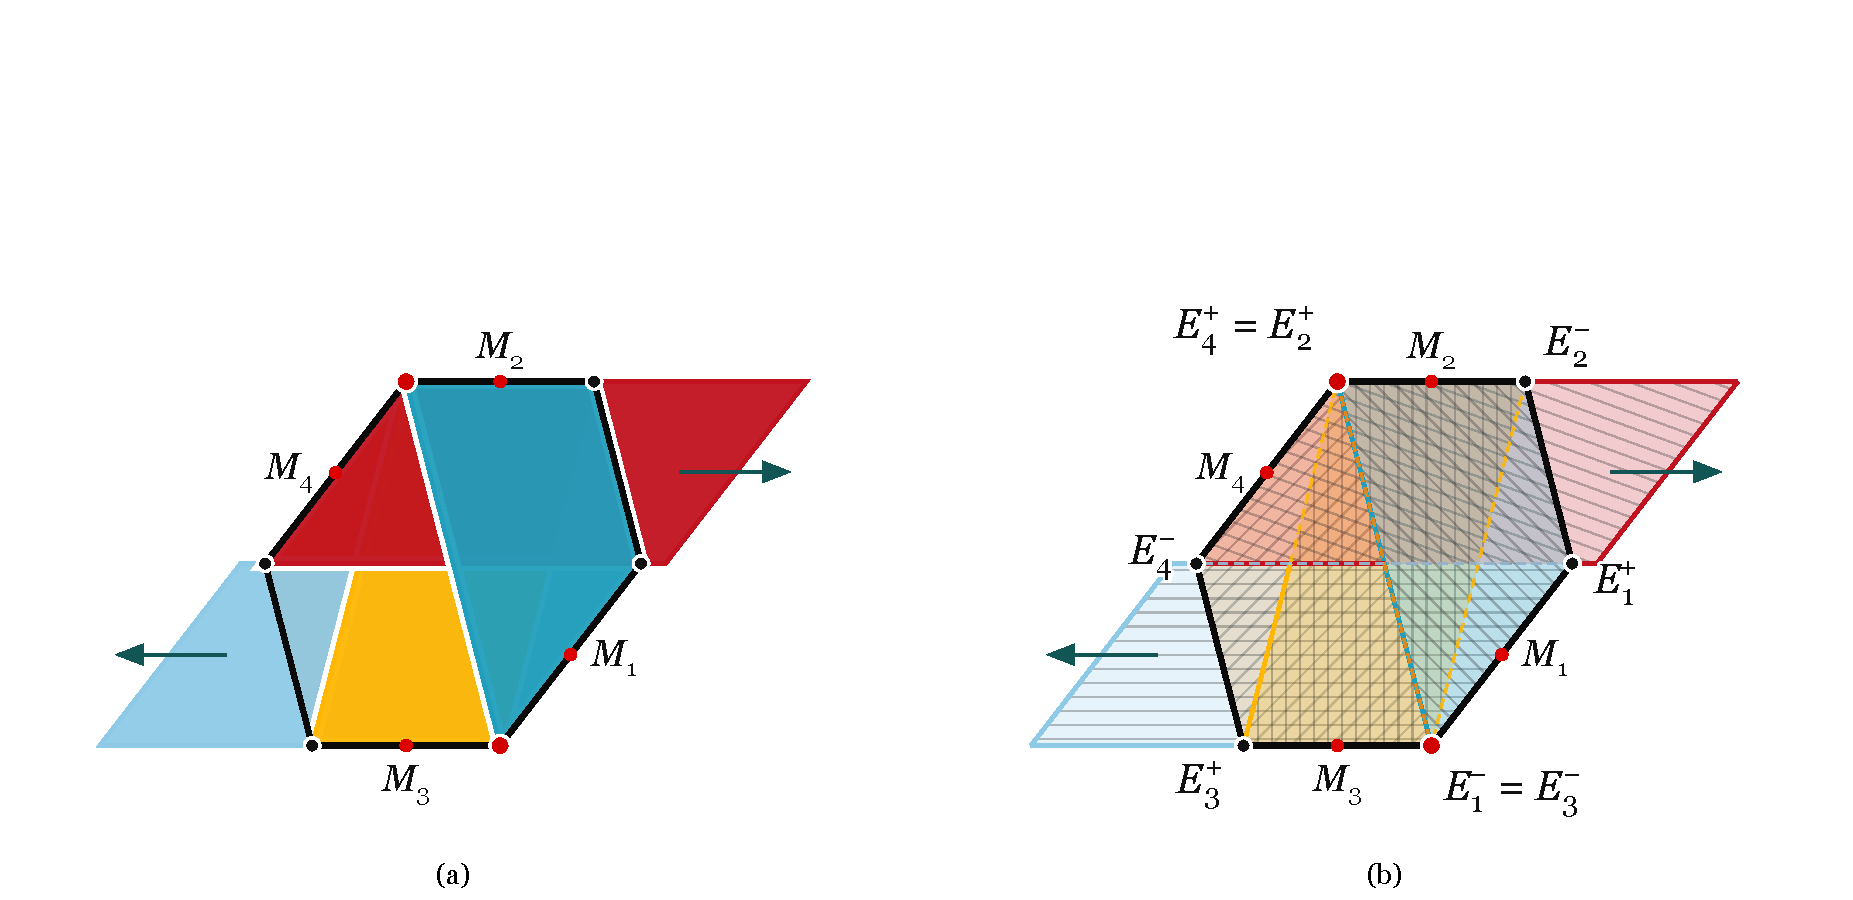
\includegraphics[width=0.85\linewidth]{figs/fig41-tight.pdf}
\caption{The exact figure-eight contact-chamber minimizer $\theta^*_{4_1}$. The core outline (heavy) is the centrally symmetric hexagon of Theorem~\ref{mainthm:hex}; its six sides are the four crease chords together with two band-edge segments, and the two red vertices are the double points $E_2^+=E_4^+$ and $E_1^-=E_3^-$ at which the crease chords close into a chain. The tails (arrows) leave in opposite directions, flush along the shared edge $y=\tfrac12$. All vertex coordinates lie in $\Q(\sqrt{15})$.}
\label{fig:f8tight}
\end{figure}

The shape describes the certified figure-eight contact-chamber minimizer (Figure~\ref{fig:f8tight}). The core outline is the hexagon with vertices
\begin{gather*}
\big({-}\tfrac{13\sqrt{15}}{30},\tfrac12\big),\qquad
\big({-}\tfrac{7\sqrt{15}}{30},\tfrac32\big),\qquad
\big(\tfrac{\sqrt{15}}{30},\tfrac32\big),\\
\big(\tfrac{\sqrt{15}}{10},\tfrac12\big),\qquad
\big({-}\tfrac{\sqrt{15}}{10},-\tfrac12\big),\qquad
\big({-}\tfrac{11\sqrt{15}}{30},-\tfrac12\big),
\end{gather*}
sides in the repeating pattern $\tfrac{2\sqrt{10}}5,\ \tfrac4{\sqrt{15}},\ \tfrac4{\sqrt{15}}$, twice around, interior angles $\arccos(-\tfrac14)\approx104.48^\circ$ at the two free crease endpoints and $\pi-\tfrac12\arccos(-\tfrac14)\approx127.76^\circ$ at the other four, perimeter $\tfrac{4\sqrt{10}}5+\tfrac{16}{\sqrt{15}}$, and area $\tfrac{4\sqrt{15}}5=\tfrac35\core(\theta^*_{4_1})$. It is not the regular hexagon. Its six sides are the four crease chords together with two band-edge segments, the exact four-crease analogue of the pentagon's three creases plus two edges; and the three core passes \emph{cover} it exactly, with overlap. After rescaling the $x$-coordinate by $2\sqrt{15}$, the $y$-coordinates being already rational, every vertex is rational, each panel is a convex quadrilateral whose vertices are vertices of the hexagon, so the union lies inside the hexagon. Exact inclusion--exclusion of rational areas, $12+16+12-8-8-0+0=24$, then shows the union exhausts it: no notch, by exact arithmetic, with mean overlap $\tfrac{40}{24}=\tfrac53$. The truncation length is also exact, under the same calibrated convention as for the trefoil---stubs measured to the point where each tail exits the core outline, the rule that reproduces \eqref{eq:kauffman-ratio}: each stub equals $L_1=\tfrac{2\sqrt{15}}5$ exactly, one more expression of the symmetry, giving
\[
\trunc(\theta^*_{4_1})=\tfrac{4\sqrt{15}}5+\tfrac{4\sqrt{15}}3=\tfrac{32\sqrt{15}}{15}=8.2623\ldots,
\qquad \frac{\trunc(\theta^*_{4_1})}{\core(\theta^*_{4_1})}=\frac85 .
\]
The outermost centreline crossing and the point at which a tail exits the outline give different stub lengths even for the trefoil. Cutting at the outline recovers \eqref{eq:kauffman-ratio}. For the figure-eight state the same convention gives $\tfrac{32\sqrt{15}}{15}=32/\sqrt{15}$, the value conjectured by Kauffman \cite{kauffman2004}. Theorem~\ref{mainthm:hex} establishes attainment, reachability from open valid states and strict local minimality of \emph{core length} on the stated contact chamber. For closed folded-ribbon conventions see \cite{denne2020,chen2025,yoo2026} and the crossing-number and four-page-index bounds \cite{kimnoyoo2026,yoo2026b}.

\begin{table}[tbp]
\centering\small
\renewcommand{\arraystretch}{1.15}
\begin{tabular}{p{0.58\linewidth}p{0.29\linewidth}}
\hline
\raggedright Figure-eight claim & \raggedright Verification grade\tabularnewline
\hline
\raggedright Actual-panel validity of $\theta^*_{4_1}$; hexagonal outline; core and truncation lengths & \raggedright exact\tabularnewline
\raggedright Valid opening path for $0<s\le10^{-3}$ & \raggedright exact inequalities on a continuous interval\tabularnewline
\raggedright Strict local minimum on the stated contact chamber $\mathcal C$ & \raggedright exact rank and positive KKT multipliers\tabularnewline
\raggedright Existence and uniqueness of the symmetric contact root in its specified box & \raggedright interval (Krawczyk)\tabularnewline
\raggedright Sampled cells, boundary inventory, descent endpoints and multistart KKT harvest & \raggedright numerical; finite search only\tabularnewline
\raggedright Necessity of the eight inequalities for every nearby valid state; exhaustive cell and root coverage & \raggedright not established\tabularnewline
\hline
\end{tabular}
\caption{Verification grades for the figure-eight results. The exact and interval certificates do not depend on the numerical search counts. The contact chamber $\mathcal C$ is defined by its eight explicit inequalities; the last row records the stronger statements that would extend the result beyond that chamber.}
\label{tab:figure8-grades}
\end{table}

\subsection{What the second instance teaches}
Three contrasts with the trefoil are worth stating plainly. First, the algebra collapsed: one more crossing, and the certified contact-chamber minimizer has quadratic coordinates, whereas the trefoil state has degree twelve with an associated sextic splitting group $S_6$. The trefoil's algebraic complexity occurs together with its notch---the record of a corner contact prised open along the second family---while at the figure-eight the central symmetry closes the crease chain exactly and no notch forms. These two examples suggest that the contact pattern, as well as the crossing number, matters to the algebraic complexity; they do not establish a general classification. Second, the phenomenology of the tails inverts: the tight trefoil sends its tails out at $69.5^\circ$---the $P_0P_3$ crossing angle of Remark~\ref{rem:gpaudit}---, the hexagonal figure-eight state sends them out antiparallel and flush, offset by exactly one strip width---consistent with the figure-eight's everyday use as a stopper knot that is loaded straight through. For a strip of width $w$ the prediction reads: hexagonal core with long sides $\approx1.265\,w$ and short sides $\approx1.033\,w$, consumed core material $\approx5.164\,w$, tails leaving antiparallel with zero gap. Third, both instances use the same verification grades and identify-then-verify procedure. Their geometric predicates still require separate checks: the four-crease computations use the actual oblique crease caps and unbounded tails, and their numerical searches are distinguished from the exact state and local-optimality certificates in Table~\ref{tab:figure8-grades}.

The numerical census has been rerun with the corrected actual-panel oracle. Of $4000$ boundary-probe attempts with seed $11$, $3995$ reach a boundary and all are assigned to the same eight endpoint-side contact labels; five attempts are rejected because the proposed starting state fails the current validity test. Both the boundary test and the event classification use oblique crease caps. This is a sampled inventory of the contacts active at $\theta^*_{4_1}$, not a proof that no other faces occur. Targeted minimization of $15$ crossing and length margins, from four revalidated starting states each, gives an overall observed minimum $0.5252598788\ldots$ in $56\,270$ trials. That observed value is not a global lower bound and does not exclude code walls from the valid closure.

The KKT rerun covers all $254$ nonempty subsets of at most seven of these eight contact functions, using seven initial values per subset: $1778$ Newton attempts. It returns $56$ convergence records, including repeated occurrences of the same root across seeds and subsets. Of these, $42$ have a negative multiplier and $14$ pass the nonnegative-multiplier filter; all $14$ lie within $3\times10^{-10}$ of $\theta^*_{4_1}$ in the seven chart coordinates. The residual stopping tolerance is $5\times10^{-8}$, the numerical approximate-closure distance tolerance is $10^{-6}$, and the multiplier tolerance is $10^{-8}$. Every root is checked against the actual panel oracle, independently of the sampled wall inventory. The exact candidate is validated separately below; neither convergence counts nor these numerical filters certify additional roots. Targeted searches of the other eight abstract cells, with $60$ restarts per cell and at most $4000$ steps per restart, find shadow realizations in four cells but no valid figure-eight state in any of the eight. These finite searches provide no emptiness proof. All original data, the unfiltered KKT records, final-predicate outcomes and source snapshots are retained in the ancillary repository; \texttt{scripts/reproduce-n4-search.sh} reproduces the full-size protocol.

Under the tangent half-angle substitution $u_i=\tan(\tau_i/2)$ the chart becomes rational, all eight walls become integer polynomials (degrees $7$ to $15$), the tight state keeps quadratic coordinates $u^*=(\sqrt{15}/3,\,\sqrt{15},\,-\sqrt{15},\,-\sqrt{15}/3)$ at which all eight polynomials vanish exactly, and a Krawczyk certificate on a box of radius $10^{-25}$ encloses $\theta^*_{4_1}$ with existence and uniqueness in its stratum. At the point itself validity is exact: \texttt{n4\_exact\_valid} builds all five actual panels from their side and crease half-planes, checks all six forbidden crease/pass pairs by clipping the full relative-open chord, and checks all nonadjacent centreline pairs. It uses no floating-point predicate to decide which constraints to include. Exact opening and Krawczyk certificates supplement this pointwise check; neither establishes global root coverage or all local contact branches.

The rerun leaves the proof obligations unchanged. Lemma~\ref{lem:wallcat} gives a finite \emph{candidate} catalogue of endpoint events and crease-pair contacts, but determining which occur as faces still requires per-event analysis, as performed for the trefoil in Corollary~\ref{cor:wallcomplete}. The Newton harvest does not establish per-stratum root completeness, and the sampled cells do not exhaust the geometric branch. Reachability, in contrast, is certified by Lemma~\ref{lem:slackstart41}. Extending contact-chamber optimality to the entire geometric cell requires a local tangent-cone argument at the simultaneous endpoint/cap contacts.

\section{Open problems}\label{sec:open}

\begin{enumerate}
\item\label{op:uniqueness}\emph{Proving global uniqueness.} After Theorem~\ref{thm:census} the principal numerical component is the per-stratum completeness of the harvest. The polynomialized wall system makes the exact route concrete: for $|S|=5$ the wall equations alone form a square polynomial system; for $|S|=4$ one adjoins the $\lambda$-eliminated determinant $\det[\nabla W_S\,|\,2D_p^2\nabla\ell]=0$; and for $|S|\le3$ the corresponding minor conditions. Each is a zero-dimensional system amenable to resultants, and the low-degree strata are the natural starting point. The obstruction is the trio of degree-$16$ walls $w_4,w_6,w_8$, which do however factor on partial loci, as the $N_5$ reduction already showed. A related missing ingredient is \emph{properness} of $\core$, that is, boundedness of its sublevel sets in the closure of $\M$; properness is what would turn ``a maximal pulling path converges to a tight state'' from a sketch into a theorem.

\item\label{op:lifting}\emph{Path-lifting.} Theorem~\ref{mainthm:realization} lifts individual states into slabs. Is there a theorem lifting an entire tightening path $p:[0,1]\to\M$ to a continuous family of realizations in a slab of \emph{fixed} height $\varepsilon>0$? On a compact subinterval inside an open stratum the budget $\varepsilon_0$ is continuous and positive, so one may take $\varepsilon<\min_t\varepsilon_0(p(t))$, and the ramp construction is itself a continuous function of the state; the open-interval case should reduce to a continuity statement about the existing construction, in the spirit of the monotone-path formalizations of \cite{cdr2003}. The hard end is $t\to1$: as the clearances are exhausted, the sufficient bound for this constant-height construction tends to zero. This does not rule out other realizations at the endpoint in a slab of fixed height; such an exclusion would require a separate lower-bound argument.

\item\label{op:thickness}\emph{Finite thickness.} Our realizations are $\varepsilon$-slab embeddings of a zero-thickness surface. A genuinely thick model---positive reach, a tubular neighbourhood of the sheet, contact forces in the sense of \cite{svdm2004,cks2002}---is a different and harder object. The relation between the two, and the correct notion of tightness for the thick model, is open.

\item\label{op:generaln}\emph{General $n$.} Which other four-crease cells contain tight states? The rational half-angle chart gives polynomial contact equations for comparing them with the certified hexagon. For $n\ge5$ the questions include the dimension, the wall catalogue, and whether truncation and core length select different states. Comparisons with closed ribbons \cite{denne2020,chen2025} require matching the length and closure conventions.

\item\label{op:creases}\emph{The complete-crease assumption.} We assume throughout that every crease is a chord joining the two long edges. Partial creases---corner folds---are excluded by a modelling decision, in line with the standard layer formalisms \cite{justin1997,hull2002,demaine2007}; whether they can matter for tying or for tightening is open.

\item\label{op:order}\emph{Sheet versus pointwise induced order.} Our definition of realization uses sheet separation. The pointwise form, comparing the heights of overlapping material points, is not known to be equivalent, and the pathology to exclude is a realization that pleats vertically inside the slab, through which the mod-$2$ argument behind the converse could leak. Two related gaps: strong $\varepsilon$-realization at a \emph{fixed} small $\varepsilon$ for a zero-clearance state, where the constant-height construction fails and a wedge-shaped height assignment is the natural candidate; and the formalization of the mod-$2$ crossing-parity lemma, whose proof uses standard mod-$2$ intersection theory \cite{gp1974} and which is the main target in formalizing the realization theory.

\item\label{op:kauffman}\emph{Kauffman's global conjecture.} Theorem~\ref{mainthm:kauffman} is local and confined to the three-crease branch. The global statement---that $4/\sqrt{5-2\sqrt5}$ is the minimum of $L/W$ over all flattened truncated trefoil ribbons \cite{kauffman2004}---is untouched. A natural intermediate step is to compare against branches with more creases, where the closed-ribbon results suggest that extra folds help for the closed functional; the immersed analogues \cite{immersed2020,ayala2025}, in which vertex tension balance plays the role of our wall-KKT balance, are the other obvious source of technique.

\item\label{op:formal}\emph{Formalization.} Sixteen algebraic core statements are machine-checked (Appendix~\ref{app:lean}). The bridge from that algebra to the geometry---coordinates, material topology, layer order, wall definitions---is not formalized, and the mod-$2$ crossing-parity lemma, standard in content \cite{gp1974}, is the identified hard case for formalization.
\end{enumerate}

\appendix

\section{The verification suite}\label{app:suite}

Structural claims were first explored numerically in double precision and then promoted through higher-precision evaluation ($40$--$80$ digits), algebraic identification, exact quotient-field verification, interval arithmetic for existence and signs, and Lean~4 proofs for the supporting algebraic core. Integer-relation detection \cite{fba1999} served only as a search heuristic; every candidate expression it proposed was either verified as an exact identity or discarded.

Exact verification is carried out in the quotient field $\Q[x]/(p_x)$, and in $\Q(x_0)$ or $\Q(x)$ where the pentagon or a general state is concerned, without heuristic numerical simplification (\texttt{nsimplify}) or floating-point sign calibration. A recursive evaluator reduces rational expressions to canonical representatives modulo the minimal polynomial, so claimed identities are decided by exact reduction to $0$ rather than tolerance checks. For inequalities and existence assertions we use outward-rounded interval arithmetic \cite{neumaier1990}: Krawczyk and interval-Newton enclosures on boxes of radius $10^{-20}$ to $10^{-50}$ at $40$- to $80$-digit precision, together with interval evaluation for positivity of multipliers, the reduced Hessian, and census wall margins. The mutation suite (\texttt{test\_guards}) runs ten original certificates and their altered copies in default and optimized Python. Each altered copy must exit with its expected mathematical diagnostic. Structurally important computations are cross-checked by independent routes---rational expression trees versus polynomialized walls, symbolic differentiation versus an $80$-digit second difference (agreeing to $4.7\times10^{-34}$), and \texttt{mpmath} versus \textsc{Arb} ball arithmetic (\texttt{arb\_recheck}).

Table~\ref{tab:suite} lists the principal certificate for each result. The historical probes in the reproducibility guide include the endpoint-sampling counterexample of Remark~\ref{rem:methods}.

The companion distribution \cite{anc} contains the source files and dependency locks, the recorded numerical checkpoints, and SHA-256 manifests for the calculations, logs and artifacts.

\begin{table}[tbp]
\centering\small
\renewcommand{\arraystretch}{1.15}
\begin{tabular}{@{}>{\raggedright\arraybackslash}p{0.445\linewidth}@{\hspace{0.035\linewidth}}>{\raggedright\arraybackslash}p{0.52\linewidth}@{}}
\hline
Result and scope & Principal verification scripts\\
\hline
A. Alternating trefoil word, slope signs and local/global layer order &
\texttt{check\_gauss}, \texttt{check\_gp}, \texttt{exact\_common\_overlap}\\
B. Slice identities, chart and contact walls &
\texttt{exact\_slice}, \texttt{exact\_taco}, \texttt{exact\_common\_overlap}\\
C. Inward slope $-1/20$, monotone descent and crossing preservation &
\texttt{exact\_core\_descent}, \texttt{exact\_reach}, \texttt{exact\_branch}\\
D. Degree twelve, stationarity and positive reduced curvature at $\td$ &
\texttt{exact\_field}, \texttt{exact\_unique\_h}, \texttt{exact\_kkt\_dagger}, \texttt{exact\_second}\\
D and Section~\ref{sec:shape}. Seven-sided outline and notch &
\texttt{exact\_outline}, \texttt{exact\_notch}\\
E. Truncation minimum and flush-cut edges at $P^*$ &
\texttt{exact\_kauffman2}, \texttt{exact\_trunc\_nbhd}\\
F. Opening at both distinguished states and the cyclic local-order example &
\texttt{exact\_opening}, \texttt{exact\_common\_overlap}\\
G. Wall exclusion on $72$ isolated root boxes and classification of $32$ inconclusive centres &
\texttt{exact\_census\_roots} (Arb), using the saved harvest from \texttt{uniq\_census}\\
H. Figure-eight validity, opening, stationarity, chamber minimum and hexagon &
\texttt{n4\_exact\_valid}, \texttt{n4\_exact\_opening}, \texttt{n4\_exact\_kkt}, \texttt{n4\_exact\_local}, \texttt{n4\_krawczyk}, \texttt{n4\_certify}\\
H. Combinatorial enumeration and recorded numerical search &
\texttt{n4\_cells3}, \texttt{check\_n4\_geometry}, \texttt{check\_n4\_rerun}\\
\hline
\end{tabular}
\smallskip\caption{Computational evidence for Theorems A--H. The reproducibility guide gives the commands, inputs and expected results. The last row includes a finite numerical search.}
\label{tab:suite}
\end{table}

\FloatBarrier
\section{Lean formalization}\label{app:lean}

Sixteen statements forming the algebraic core of the paper are machine-checked in Lean~4 against Mathlib \cite{mathlib2020}, in two files. The nine theorems of \texttt{Pentagon.lean} formalize the slice: the closed form of the gap $\Delta$, the sum-of-squares identity behind the positivity of the numerator of $\Delta'$, the strict positivity of the slice polynomial $p$ on $y>0$, the characterization and the uniqueness of the contact root in the relevant range, the implication from that root to $|EH|^2=|EF|^2$, a root-of-unity closure lemma, and the closed form and strict monotonicity of $\core$ along the slice---together, supporting algebra for the folklore half of Theorem~\ref{mainthm:pass}, without a formal polygon or angle model. The seven theorems of \texttt{ThetaDagger.lean} formalize the second family: the field identity $\ell=h+b$ as an exact equality of polynomials, the monotonicity package for the defining polynomial, existence of its root in $(0.32,0.33)$ by the intermediate value theorem together with uniqueness in $(0,1)$, and the certificate separating the pentagon from $\td$, discharged by \texttt{linear\_combination} on explicit certificate polynomials. Table~\ref{tab:lean} lists them; there, $P(x)=5x^4-10x^2+1$ is the pentagon contact polynomial, $p$ denotes the slice polynomial in $y=x^2$ in the \texttt{Pentagon} rows and the defining polynomial of the second family in the \texttt{ThetaDagger} rows, and equal statement names in the two files are distinct namespaced theorems.

\begin{table}[t]
\centering\small
\begin{tabular}{@{}ll@{}}
\hline
Theorem & Content\\
\hline
\multicolumn{2}{@{}l}{\emph{\texttt{Pentagon.lean}}, nine theorems}\\
\texttt{delta\_formula} & closed form of the gap $\Delta$\\
\texttt{deriv\_numerator\_pos} & positivity of the numerator of $\Delta'$ (SOS identity)\\
\texttt{p\_pos} & $p(y)>0$ for $y>0$\\
\texttt{x0\_root} & $s^2=5$ and $sx^2=s-2$ imply $P(x)=0$\\
\texttt{root\_unique} & uniqueness of the root in the range $y<\frac13$\\
\texttt{side\_eq\_of\_contact} & $P(x)=0$ implies $((1-3x^2)/(2x))^2=1+x^2$\\
\texttt{closure\_root\_of\_unity} & $1+z+\dots+z^4=0$ implies $z^5=1$\\
\texttt{ell\_core\_closed\_form} & $\core=\frac1x-x$ on the slice\\
\texttt{ell\_core\_strict\_anti} & strict decrease of $\core$ along the slice\\
\hline
\multicolumn{2}{@{}l}{\emph{\texttt{ThetaDagger.lean}}, seven theorems}\\
\texttt{ell\_eq\_h\_add\_b} & the identity $\ell=h+b$ as an equality in $\Q[x]$\\
\texttt{deriv\_pos} & $p'>0$ on $(0,1]$\\
\texttt{p\_hasDerivAt} & the derivative formula for $p$\\
\texttt{p\_strictMonoOn} & $p$ strictly increasing on $[0,1]$\\
\texttt{root\_exists} & existence of a root in $(0.32,0.33)$\\
\texttt{root\_unique} & uniqueness of that root in $(0,1)$\\
\texttt{pentagon\_not\_thetaDagger} & the saddle--well separation certificate\\
\hline
\end{tabular}
\caption{The sixteen machine-checked statements, grouped by file.}
\label{tab:lean}
\end{table}

What is machine-checked is the \emph{algebraic} content of these statements. The bridge from that algebra to the geometry of a folded strip---the coordinate setup, the material topology, the layer order, the wall definitions---remains human proof supported by exact symbolic derivation. Formalizing that bridge is a large project; it is not claimed here, and its identified hard case is recorded as open problem~\ref{op:formal}.
